\documentclass[11pt,a4paper]{article}

\usepackage[margin=2.5cm]{geometry}
\usepackage{amsmath,amssymb,amsthm}
\usepackage{mathtools}
\usepackage{booktabs}
\usepackage{enumitem}
\usepackage{hyperref}
\usepackage{xcolor}
\usepackage{listings}
\usepackage{algorithm}
\usepackage{algpseudocode}
\usepackage{tikz}
\usetikzlibrary{arrows.meta,positioning,decorations.pathreplacing}

\hypersetup{
    colorlinks=true,
    linkcolor=blue!60!black,
    citecolor=blue!60!black,
    urlcolor=blue!60!black,
}

\lstset{
    language=Python,
    basicstyle=\ttfamily\small,
    keywordstyle=\color{blue!70!black}\bfseries,
    commentstyle=\color{green!50!black}\itshape,
    stringstyle=\color{red!60!black},
    numbers=left,
    numberstyle=\tiny\color{gray},
    numbersep=6pt,
    frame=single,
    framerule=0.4pt,
    rulecolor=\color{gray!50},
    breaklines=true,
    breakatwhitespace=true,
    showstringspaces=false,
    tabsize=4,
    xleftmargin=1.5em,
    framexleftmargin=1.5em,
    aboveskip=1em,
    belowskip=1em,
    morekeywords={function,end,for,if,else,elseif,return,struct,mutable,
                  @threads,@inbounds,@inline,@printf,Float64,Int,Bool,
                  Vector,Matrix,true,false,nothing,clamp,max,min,abs,copy},
}

%% ---- FIX: wrap both macros in \mathord so outer ^ and _ attach to the
%%           whole atom, not to the bare "p" that already carries a superscript.
\newcommand{\pstar}{\mathord{p^{*}}}
\newcommand{\poj}{\mathord{p^{\mathrm{oj}}}}
\newcommand{\supnorm}[1]{\lVert #1 \rVert_\infty}
\newcommand{\code}[1]{\texttt{#1}}

\theoremstyle{definition}
\newtheorem{problem}{Problem}
\newtheorem{fix}{Fix}

\title{\textbf{Resolving the Period-2 Limit Cycle in the\\Skilled Block Cutoff Iteration}\\[0.5em]
\large Technical Note --- Segmented Search Model Solver}
\author{}
\date{March 2026}

\begin{document}

\maketitle
\thispagestyle{empty}

\begin{abstract}
\noindent
The skilled-block outer loop in the segmented search model solver exhibits a
period-2 limit cycle in the reservation-quality cutoff $\pstar_S(x)$ and OJS
cutoff $\poj(x)$, even as market tightness $\theta_S$ converges.  This note
documents the root cause---a discontinuous surplus map created by hard
grid-thresholding in the inner loop---and describes two complementary fixes:
(i)~soft thresholding of the surplus surfaces at the cutoff boundary, and
(ii)~Anderson acceleration on the full joint state vector
$[\theta;\, \pstar;\, \poj]$.
\end{abstract}

\tableofcontents

\newpage

%% ========================================================================
\section{Symptom}
%% ========================================================================

The skilled-block outer loop alternates between exactly two states on every
iteration:
%
\begin{center}
\begin{tabular}{lcc}
\toprule
Iteration & $\Delta \pstar$ & $\Delta \poj$ \\
\midrule
odd  & 0.9828 & 0.9848 \\
even & 0.4091 & 0.4120 \\
\bottomrule
\end{tabular}
\end{center}
%
Meanwhile $\Delta\theta = 0$ to machine precision.  The pattern persists
indefinitely regardless of damping parameter $\delta \in (0,1]$ applied to
the cutoff update:
\[
    \pstar_S^{(n+1)}(x) \;=\; \delta\, \hat{p}^{(n)}(x)
                          \;+\; (1-\delta)\, \pstar_S^{(n)}(x).
\]
Heavy damping ($\delta \ll 1$) slows the cycle but does not break it.  This
is because the underlying fixed-point map is \emph{discontinuous}: no convex
combination of a discontinuous map with the identity can produce a
contraction.


%% ========================================================================
\section{Architecture of the Skilled-Block Solver}
%% ========================================================================

The outer loop iterates on the state $(\theta_S,\, \pstar_S,\, \poj)$ as
follows:

\begin{enumerate}[label=\textbf{(\Alph*)}]
    \item \textbf{Inner loop.}  Given $(\theta_S,\, \pstar_S,\, \poj)$,
          solve for unemployment values $U_S(x)$ and surplus surfaces
          $S^0(x,p)$, $S^1(x,p)$ on the $(x,p)$ grid.

    \item \textbf{Cutoff update.}  Read off new cutoffs from the surplus
          surfaces:
    \begin{align}
        \hat{p}^{*}(x) &= \inf\bigl\{ p :
            \max\bigl(S^0(x,p),\, S^1(x,p)\bigr) \geq 0 \bigr\},
            \label{eq:pstar-def}\\
        \hat{p}^{\mathrm{oj}}(x) &= \inf\bigl\{ p \geq \pstar(x) :
            S^1(x,p) - S^0(x,p) \leq 0 \bigr\}.
            \label{eq:poj-def}
    \end{align}

    \item \textbf{Stationary distribution.}  Compute
          $(u_S(x),\, e_S(x,p))$ given the new cutoffs.

    \item \textbf{Free entry.}  Update $\theta_S$ via the free-entry
          condition $k = q(\theta_S)\, \bar{J}$.
\end{enumerate}

The convergence criterion checks
$d = \max(\lvert\Delta\theta\rvert,\, \supnorm{\Delta \pstar},\,
\supnorm{\Delta \poj})$.


%% ========================================================================
\section{Root Cause: Discontinuous Surplus Map}
\label{sec:root-cause}
%% ========================================================================

\subsection{The hard-threshold mechanism}

In step~(A), the inner loop uses \code{pcut\_index(pgrid, pstar)} to find the
first grid node $j_0$ such that $p_{j_0} \geq \pstar_S(x)$.  All surplus
entries below $j_0$ are hard-zeroed:
%
\begin{equation}
    J^0(x, p_j) = J^1(x, p_j) = 0 \qquad \text{for } j < j_0.
    \label{eq:hard-zero}
\end{equation}
%
Since $j_0 = \lceil \pstar_S \rceil_{\text{grid}}$ is a step function of
$\pstar_S$, the surplus surfaces $S^0, S^1$ are \emph{discontinuous} in
$\pstar_S$.  Concretely, for a grid spacing $\Delta p \approx 0.012$
(80-point Gauss--Legendre on $[0,1]$):
%
\begin{itemize}
    \item Moving $\pstar_S$ from $p_{j_0} - \varepsilon$ to
          $p_{j_0} + \varepsilon$ causes $j_0$ to jump from $j_0$ to
          $j_0 + 1$.
    \item This zeros out an additional row of the surplus, discretely
          changing the tail integral $I(x)$ and the unemployment value
          $U_S(x)$.
    \item The new surplus surface yields a cutoff $\hat{p}^{*}$ that
          jumps back across the boundary.
\end{itemize}

\subsection{Why $\theta$ converges but $\pstar$ does not}

Market tightness $\theta_S$ is determined by the free-entry condition
\[
    k = q(\theta_S)\, \bar{J}, \qquad
    \bar{J} = \frac{\sum_{x} w_x \bigl[u_S(x)\, \tilde{J}(x) +
                    \cdots\bigr]}
                   {\sum_{x} w_x \bigl[u_S(x) + \cdots\bigr]},
\]
which aggregates over all worker types $x$.  The grid-snapping
discontinuities in individual $\pstar_S(x)$ values are averaged out in this
integral, producing a smooth function of the state.  Hence $\theta_S$
converges.

By contrast, $\pstar_S(x)$ for each $x$ is directly exposed to the
discontinuity.  The map $\pstar^{(n)} \mapsto \pstar^{(n+1)}$ has a jump at
each grid node, and the fixed point lies in a gap between two grid-aligned
attractors.

\subsection{The period-2 attractor}

\begin{figure}[h]
\centering
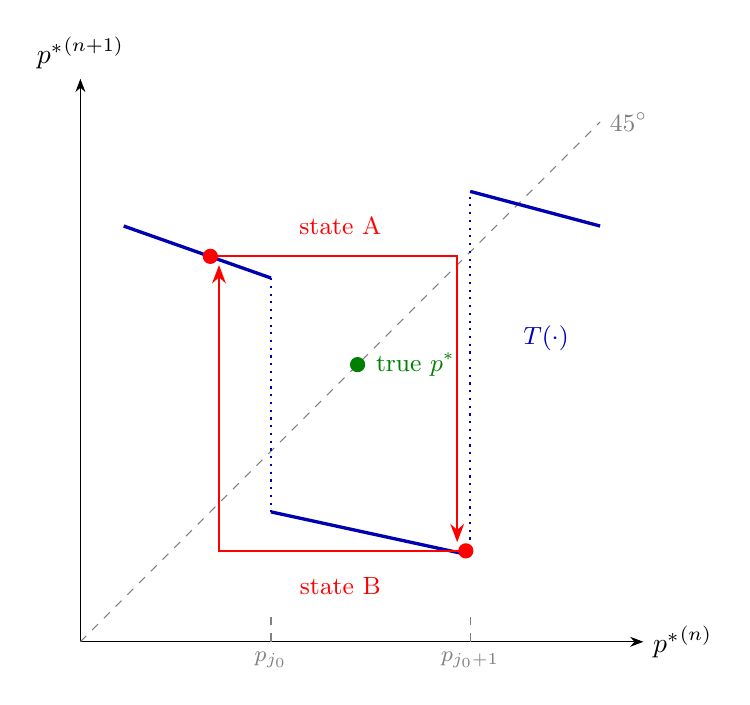
\begin{tikzpicture}[>=Stealth, scale=1.1]
    % Axes
    \draw[->] (0,0) -- (6.5,0) node[right] {$\pstar^{(n)}$};
    \draw[->] (0,0) -- (0,6.5) node[above] {$\pstar^{(n+1)}$};
    \draw[dashed, gray] (0,0) -- (6,6)
        node[right, gray, font=\small] {$45^\circ$};

    % The discontinuous map (schematic)
    \draw[blue!70!black, very thick]
        (0.5, 4.8) -- (2.2, 4.2);
    \draw[blue!70!black, very thick]
        (2.2, 1.5) -- (4.5, 1.0);
    \draw[blue!70!black, very thick]
        (4.5, 5.2) -- (6.0, 4.8);

    % Jump markers
    \draw[blue!70!black, dotted, thick] (2.2, 4.2) -- (2.2, 1.5);
    \draw[blue!70!black, dotted, thick] (4.5, 1.0) -- (4.5, 5.2);

    % Grid node labels
    \draw[gray, dashed] (2.2, 0) -- (2.2, 0.3);
    \node[below, gray, font=\footnotesize] at (2.2, 0) {$p_{j_0}$};
    \draw[gray, dashed] (4.5, 0) -- (4.5, 0.3);
    \node[below, gray, font=\footnotesize] at (4.5, 0) {$p_{j_0+1}$};

    % Period-2 orbit
    \fill[red] (1.5, 4.45) circle (2.5pt);
    \fill[red] (4.45, 1.05) circle (2.5pt);
    \draw[->, red, thick] (1.5, 4.45) -- (4.35, 4.45) -- (4.35, 1.15);
    \draw[->, red, thick] (4.45, 1.05) -- (1.6, 1.05) -- (1.6, 4.35);

    \node[red, font=\small] at (3.0, 4.8) {state A};
    \node[red, font=\small] at (3.0, 0.65) {state B};

    % True fixed point
    \fill[green!50!black] (3.2, 3.2) circle (2.5pt);
    \node[green!50!black, font=\small, right] at (3.3, 3.2) {true $\pstar$};

    % Label
    \node[blue!70!black, font=\small, right] at (5.0, 3.5) {$T(\cdot)$};
\end{tikzpicture}
\caption{Schematic of the discontinuous cutoff map
  $T\colon \pstar^{(n)} \mapsto \pstar^{(n+1)}$.
  The jumps at grid nodes $p_{j_0}$ and $p_{j_0+1}$ create a period-2 orbit
  (red arrows) that traps the iteration.  The true fixed point (green) lies
  in the gap and is unreachable by simple iteration.}
\label{fig:limit-cycle}
\end{figure}

%% ========================================================================
\section{Fix 1: Soft Thresholding in the Inner Loop}
\label{sec:soft-threshold}
%% ========================================================================

\subsection{Idea}

Replace the hard threshold~\eqref{eq:hard-zero} with a smooth weight
$\omega_j \in [0,1]$ that represents the fraction of the quadrature cell
around node $j$ that lies above $\pstar_S(x)$.  This makes the surplus
surfaces a \emph{continuous} function of $\pstar_S$, eliminating the
discontinuity that drives the limit cycle.

\subsection{Definition of $\omega_j$}

For grid node $j$ with value $p_j$ and cutoff $\pstar$:
%
\begin{equation}
    \omega_j(\pstar) =
    \begin{cases}
        1 & \text{if } p_j \geq \pstar, \\[4pt]
        \displaystyle\frac{p_{j+1} - \pstar}{p_{j+1} - p_j}
          & \text{if } p_j < \pstar < p_{j+1}, \\[8pt]
        0 & \text{if } p_{j+1} \leq \pstar,
    \end{cases}
    \label{eq:soft-weight}
\end{equation}
%
where $p_{j+1}$ is the next grid node.  The key properties are:
%
\begin{enumerate}[label=(\roman*)]
    \item $\omega_j$ is \emph{continuous} in $\pstar$ (piecewise linear).
    \item $\omega_j$ agrees with the hard threshold at grid nodes:
          $\omega_j(p_k) = \mathbf{1}[j \geq k]$ for all grid nodes $p_k$.
    \item Only one node (the ``straddling'' node) gets a fractional weight;
          all others get 0 or 1.
    \item As the grid is refined ($\Delta p \to 0$),
          $\omega_j \to \mathbf{1}[p_j \geq \pstar]$.
\end{enumerate}

\subsection{Modified inner loop equations}

The tail integral becomes:
\begin{equation}
    I(x) = \sum_{j=1}^{N_p} \omega_j(\pstar_S(x)) \cdot
            \frac{\max\bigl(J^0(x,p_j),\, J^1(x,p_j)\bigr)}{1-\beta}
            \cdot \gamma(p_j)\, w_j,
\end{equation}
and the surplus values are scaled:
\begin{align}
    J^0(x, p_j) &= (1-\beta)\, \omega_j\, S^0(x, p_j), \\
    J^1(x, p_j) &= (1-\beta)\, \omega_j\, S^1(x, p_j), \\
    E^0(x, p_j) &= U_S(x) + \beta\, \omega_j\, S^0(x, p_j), \\
    E^1(x, p_j) &= U_S(x) + \beta\, \omega_j\, S^1(x, p_j),
\end{align}
where $S^0, S^1$ are computed with the same formulas as before.  The
multiplication by $\omega_j$ smoothly interpolates between the active
($\omega_j = 1$) and inactive ($\omega_j = 0$) states.

\subsection{Implementation}

\begin{lstlisting}
@inline function _soft_weight(pj, pstar, pgrid, j, Np)
    pj >= pstar && return 1.0
    j >= Np && return 0.0
    p_next = pgrid[min(j + 1, Np)]
    p_next <= pstar && return 0.0
    cell = p_next - pj
    cell < 1e-14 && return 0.0
    return clamp((p_next - pstar) / cell, 0.0, 1.0)
end
\end{lstlisting}

This is called for every $(x, j)$ pair in the inner loop.  The overhead is
minimal: one comparison and one division per grid node.

\subsection{Effect on the cutoff map}

With soft thresholding, moving $\pstar_S$ across a grid node boundary no
longer causes a discontinuous jump in the surplus.  Instead, the surplus at
the straddling node transitions linearly from its full value to zero.  The
composition
\[
    T:\; \pstar^{(n)}
    \;\xrightarrow{\text{inner loop}}\; (S^0, S^1)
    \;\xrightarrow{\text{zero-crossing}}\; \pstar^{(n+1)}
\]
is now a \emph{continuous} map, for which standard fixed-point theory
(Brouwer, contraction mapping) applies.

%% ========================================================================
\section{Fix 2: Joint Anderson Acceleration}
\label{sec:anderson}
%% ========================================================================

\subsection{Motivation}

Even with the soft threshold, the map $T$ may have a spectral radius close
to 1 near the fixed point, leading to slow convergence.  Anderson
acceleration (mixing) with memory $m=1$ is particularly effective at
breaking period-2 cycles because it computes the optimal linear combination
of the two most recent iterates.

\subsection{Prior state}

The original code applied Anderson acceleration to $\theta_S$
\emph{only}---a scalar.  The cutoffs $\pstar_S(x)$ and $\poj(x)$ were
updated by damped Picard iteration, which cannot break a period-2 cycle in a
high-dimensional vector.

\subsection{Joint state vector}

Define the joint state:
\[
    \mathbf{z} = \begin{pmatrix}
        \theta_S \\
        \pstar_S(x_1) \\ \vdots \\ \pstar_S(x_{N_x}) \\
        \poj(x_1)     \\ \vdots \\ \poj(x_{N_x})
    \end{pmatrix} \in \mathbb{R}^{1 + 2N_x}.
\]
The outer loop computes
$\mathbf{z}^{(n)} \mapsto \mathbf{f}^{(n)} = T(\mathbf{z}^{(n)})$ (the raw
updated state after steps A--D).  Anderson($m=1$) then sets:
\begin{align}
    \mathbf{r}^{(k)} &= \mathbf{f}^{(k)} - \mathbf{z}^{(k)}, \\
    \alpha &= -\frac{(\mathbf{r}^{(k-1)})^{\top}
                     (\mathbf{r}^{(k)} - \mathbf{r}^{(k-1)})}
                    {\lVert \mathbf{r}^{(k)} - \mathbf{r}^{(k-1)}
                     \rVert^2}, \\
    \mathbf{z}^{(k+1)} &= \alpha\, \mathbf{f}^{(k)}
                        + (1-\alpha)\, \mathbf{f}^{(k-1)}.
\end{align}

For a period-2 cycle where $\mathbf{f}^{(k)} \approx \mathbf{z}^{(k-1)}$
and $\mathbf{f}^{(k-1)} \approx \mathbf{z}^{(k)}$, this yields
$\alpha \approx 0.5$, placing the next iterate at the midpoint of the two
cycle states---which is the fixed point.

\subsection{Constraint enforcement}

After the Anderson update, we project back to the feasible set:
\begin{align}
    \theta_S       &\leftarrow \max(\theta_S,\, 10^{-14}), \\
    \pstar_S(x)    &\leftarrow \mathrm{clamp}(\pstar_S(x),\, 0,\, 1), \\
    \poj(x)        &\leftarrow \max\bigl(\pstar_S(x),\,
                                \mathrm{clamp}(\poj(x),\, 0,\, 1)\bigr).
\end{align}

%% ========================================================================
\section{Fix 3: Interpolated Cutoff Finder (Supplementary)}
\label{sec:interpolation}
%% ========================================================================

The outer-loop cutoff finder \code{find\_cutoff\_from\_j0} previously
returned the $p$-value of the first grid node where $S^{\max} \geq 0$.
This grid-snapping added $O(\Delta p)$ noise on top of any other issues.

The updated version linearly interpolates between the last negative and
first non-negative node:
\begin{equation}
    \pstar \approx p_{j^{-}} +
    \frac{-S^{\max}(p_{j^{-}})}{S^{\max}(p_{j^{+}}) - S^{\max}(p_{j^{-}})}
    \cdot (p_{j^{+}} - p_{j^{-}}),
\end{equation}
where $j^{-}$ is the last node with $S^{\max} < 0$ and
$j^{+} = j^{-} + 1$ is the first with $S^{\max} \geq 0$.

The same interpolation is applied to
\code{find\_poj\_from\_diff\_grid} for the OJS cutoff.

While this alone is insufficient to break the limit cycle (the inner loop's
hard threshold is the dominant discontinuity), it provides a smoother signal
to the outer loop once the inner loop is also smooth.

%% ========================================================================
\section{Fix 4: Restored Convergence Criterion}
\label{sec:conv-criterion}
%% ========================================================================

The convergence check in the outer loop had been modified to only check
$\theta$:
\begin{lstlisting}
# d = max(d_theta, dp, dj)  # original (commented out)
d = d_theta                  # only checks theta
\end{lstlisting}
This masked the non-convergence of $\pstar$ and $\poj$.  The full criterion
is restored:
\begin{equation}
    d = \max\bigl(\lvert\Delta\theta_S\rvert,\;
                  \supnorm{\Delta \pstar_S},\;
                  \supnorm{\Delta \poj}\bigr).
\end{equation}


%% ========================================================================
\section{Summary of Changes}
%% ========================================================================

All changes are confined to \code{skilled.jl}.  No changes to data
structures, parameter files, or the global solver loop.

\begin{center}
\renewcommand{\arraystretch}{1.3}
\begin{tabular}{@{}p{3.5cm}p{4.5cm}p{5cm}@{}}
\toprule
\textbf{Component} & \textbf{Before} & \textbf{After} \\
\midrule
Inner loop surplus thresholding &
Hard zero: $J = 0$ for $j < j_0$ &
Soft weight: $J = \omega_j \cdot (1{-}\beta) S$ with
$\omega_j \in [0,1]$ continuous in $\pstar$ \\

Anderson target &
Scalar $\theta_S$ only &
Joint $[\theta_S;\, \pstar_S;\, \poj] \in \mathbb{R}^{1+2N_x}$ \\

Cutoff finder &
Grid-snap: return $p_{j_0}$ &
Interpolated zero-crossing between $p_{j^{-}}$ and $p_{j^{+}}$ \\

Convergence check &
$d = \lvert\Delta\theta\rvert$ &
$d = \max(\lvert\Delta\theta\rvert,\,
         \supnorm{\Delta \pstar},\, \supnorm{\Delta \poj})$ \\

NaN guard &
Checks $\theta$ only &
Checks $\theta$, $\pstar$, and $\poj$ \\
\bottomrule
\end{tabular}
\end{center}


%% ========================================================================
\section{Expected Behaviour After Fix}
%% ========================================================================

\begin{enumerate}
    \item The surplus surfaces are now continuous in $\pstar_S$, so the
          fixed-point map $T$ is continuous.
    \item Anderson acceleration on the joint state will converge in $O(1)$
          iterations for any residual near-periodicity.
    \item $\theta_S$ convergence should be unaffected (it was already
          smooth).
    \item As the grid is refined ($N_p \to \infty$), the soft threshold
          converges to the hard threshold, so the solution is
          grid-consistent.
    \item The SMM objective function should see fewer solver failures (the
          non-convergence of $\pstar$ was causing
          \code{SolveResult.ok = false} for many parameter draws).
\end{enumerate}


\end{document}